\documentclass[UTF8,a4paper,12pt]{ctexart}

\usepackage[left=2.3cm,right=2.3cm,top=2.6cm,bottom=2.6cm]{geometry}
\usepackage{amsmath,amssymb,bm}
\usepackage{booktabs}
\usepackage{float}
\usepackage{graphicx}
\usepackage{hyperref}
\usepackage{caption}
\usepackage{enumitem}
\usepackage{tikz}
\usetikzlibrary{positioning,shapes,arrows.meta}

\hypersetup{
  colorlinks=true,
  linkcolor=blue,
  citecolor=blue,
  urlcolor=blue
}

\title{\textbf{倒立摆连续控制中Reward延迟影响的分析}}
\author{姓名：\underline{\hspace{3cm}} \quad 学号：\underline{\hspace{3cm}}}
\date{\today}

\begin{document}

\maketitle

\section{实验问题描述}

\subsection{任务背景}

本实验以Gymnasium框架中的\texttt{Pendulum-v1}环境为研究对象，实现Actor-Critic和DDPG两种连续控制算法，使倒立摆稳定在竖直向上的平衡位置。实验要求：
\begin{enumerate}[leftmargin=2em]
  \item 进行仿真，得到和在线教程同样的结果，并对结果进行比较分析；
  \item 说清其中的reward是怎么取的。进一步，假设系统存在5个采样周期的延迟（reward计算时只能使用5步之前的状态和输入值），重新进行仿真，输出仿真曲线，分析延迟对结果的影响。
\end{enumerate}

\subsection{环境定义}

\texttt{Pendulum-v1}的观测空间为3维连续向量$[\cos\theta, \sin\theta, \dot{\theta}]$，其中$\theta$为摆杆与竖直方向的夹角（$\theta=0$表示倒立平衡）。动作空间为1维连续量$\tau \in [-2, 2]$，表示施加在摆杆上的电机力矩。每回合最大步数为200步。

\section{Reward机制与物理尺度说明}

\subsection{环境真实Reward公式}

Pendulum-v1的即时reward由Gymnasium内置公式定义：
\begin{equation}\label{eq:true_reward}
r_{\text{true}} = -(\theta^2 + 0.1 \cdot \dot{\theta}^2 + 0.001 \cdot \tau^2)
\end{equation}

其中$\theta$为归一化角度偏差（$\theta=0$为最优，取值$\theta\in[-\pi,\pi]$），$\dot{\theta}$为角速度（取值范围$[-8,8]$），$\tau$为控制力矩（$\tau\in[-2,2]$）。最大化reward等价于让摆杆稳定在竖直位置、减少摆动并降低控制能耗。

\subsection{Reward物理尺度分析}

由于reward公式中含有平方项，不同策略下的reward数量级差异很大：

\begin{table}[H]
\centering
\caption{Pendulum-v1中Reward的物理尺度分析}
\label{tab:reward_scale}
\begin{tabular}{lccc}
\toprule
\textbf{策略类型} & \textbf{典型单步reward} & \textbf{200步累计} & \textbf{物理含义} \\
\midrule
最优策略 & $\approx -0.6$ & $\approx -120$ & $\theta\approx0,\ \dot\theta\approx0,\ \tau\approx0$ \\
随机策略 & $\approx -5.4$ & $\approx -1080$ & $\theta,\dot\theta,\tau$均匀随机 \\
劣化策略 & $\approx -7.6$ & $\approx -1520$ & 学到了推向远离平衡的错误动作 \\
\bottomrule
\end{tabular}
\end{table}

\paragraph{各分量贡献分析：}
\begin{itemize}[leftmargin=2em]
  \item 角度项$\theta^2$：$\theta\in[-\pi,\pi]$，随机时$\mathbb{E}[\theta^2] = \pi^2/3 \approx 3.29$，贡献约3.29；
  \item 角速度项$0.1\dot\theta^2$：$\dot\theta\in[-8,8]$，随机时$\mathbb{E}[\dot\theta^2] = 64/3 \approx 21.33$，贡献约2.13；
  \item 力矩项$0.001\tau^2$：$\tau\in[-2,2]$，随机时$\mathbb{E}[\tau^2] = 4/3 \approx 1.33$，贡献约0.0013。
\end{itemize}
随机策略下单步reward约$-(3.29+2.13+0.001) \approx -5.42$，200步累计约$-1084$。\textbf{因此$-1170$的累计回报表明Actor-Critic学到的策略比随机更差}——即策略梯度推向了错误的动作方向（如持续将摆杆拉离平衡位置），而这不难发生：对于基础Actor-Critic，on-policy更新的高方差使其在连续状态空间中容易陷入错误的局部最优。

\subsection{延迟Reward实现}

延迟reward的核心思想是：agent在第$t$步收到的reward来自第$t-d$步的状态和动作，而不是当前步的真实reward。实现采用FIFO队列（图~\ref{fig:delay_mechanism}）。

\begin{figure}[H]
\centering
\begin{tikzpicture}[node distance=0.6cm]
\tikzset{
    block/.style={rectangle, draw=blue!60, thick, minimum width=2.4cm, minimum height=0.7cm, align=center, fill=blue!5},
    arrow/.style={->, thick, >=Stealth},
    queue/.style={rectangle, draw=orange!70, thick, minimum width=0.9cm, minimum height=0.6cm, fill=orange!10}
}
\node[block] (env) {环境动力学};
\node[block, right=0.6cm of env] (store) {FIFO队列};
\node[queue, above=0.3cm of store] (q5) {$t-5$};
\node[queue, right=0.1cm of q5] (q4) {$t-4$};
\node[queue, right=0.1cm of q4] (q3) {$t-3$};
\node[queue, right=0.1cm of q3] (q2) {$t-2$};
\node[queue, right=0.1cm of q2] (q1) {$t-1$};
\node[queue, right=0.1cm of q1] (q0) {$t$};
\node[block, below=0.4cm of store] (reward) {计算$r_{\text{delay}}$};
\node[block, right=0.6cm of reward] (agent) {Agent $a_t$};
\draw[arrow] (env) -- node[above]{$(s_t,a_t,r_{\text{true}})$} (store);
\draw[arrow] (store) -- (reward);
\draw[arrow] (reward) -- node[above]{$r_{\text{delay}} = r(s_{t-5}, a_{t-5})$} (agent);
\draw[arrow] (agent) -- (env);
\node[font=\small, below=0.1cm of q5] {出队};
\node[font=\small, below=0.1cm of q0] {入队};
\end{tikzpicture}
\caption{延迟reward实现机制}
\label{fig:delay_mechanism}
\end{figure}

\paragraph{流程：}
\begin{enumerate}[leftmargin=2em]
  \item 环境以正常动力学推进，每步产生真实reward $r_{\text{true}}$（式~\eqref{eq:true_reward}）；
  \item 将当前步执行前的状态$s_t$和执行的动作$a_t$存入FIFO队列；
  \item 若队列长度$\leq 5$，返回$r_{\text{delay}} = 0$；否则弹出5步前的记录，用式~\eqref{eq:true_reward}重新计算reward返回agent。$info[$\text{``true\_reward''}$]$始终保存当前步真实reward用于评估。
\end{enumerate}

\section{实验设置}

\begin{table}[H]
\centering
\caption{超参数配置}
\label{tab:params}
\begin{tabular}{lll}
\toprule
\textbf{参数} & \textbf{Actor-Critic} & \textbf{DDPG} \\
\midrule
训练回合数 & 120 & 100 \\
Actor学习率 & $3\times10^{-4}$ & $1\times10^{-3}$ \\
Critic学习率 & $1\times10^{-3}$ & $2\times10^{-3}$ \\
隐藏层维度 & 128 & 128 \\
折扣因子$\gamma$ & 0.99 & 0.99 \\
经验回放 & 无 & 100,000 \\
批大小 & — & 64 \\
预热步数 & — & 1,000 \\
目标网络$\tau$ & — & 0.005 \\
\bottomrule
\end{tabular}
\end{table}

\section{仿真结果与对比分析}

\subsection{与在线教程结果对比}

以Keras官方\texttt{DDPG on Pendulum-v1}教程\footnote{\url{https://keras.io/examples/rl/ddpg_pendulum/}}为基准。

\begin{table}[H]
\centering
\caption{DDPG无延迟与Keras教程对比}
\label{tab:comparison}
\begin{tabular}{lll}
\toprule
\textbf{指标} & \textbf{Keras教程} & \textbf{本实验} \\
\midrule
初始reward & $\approx -1500$ & $-1489.58$（第10ep） \\
收敛速度 & 约40-60回合 & 第31ep达$-126.87$，第39ep达$-121.54$ \\
最终平滑reward & $-130 \sim -180$ & \textbf{$-118.36$} \\
\bottomrule
\end{tabular}
\end{table}

本实验DDPG实现与教程趋势高度一致，最终$-118.36$略优于教程基准，说明实现正确。
\begin{figure}[H]
\centering
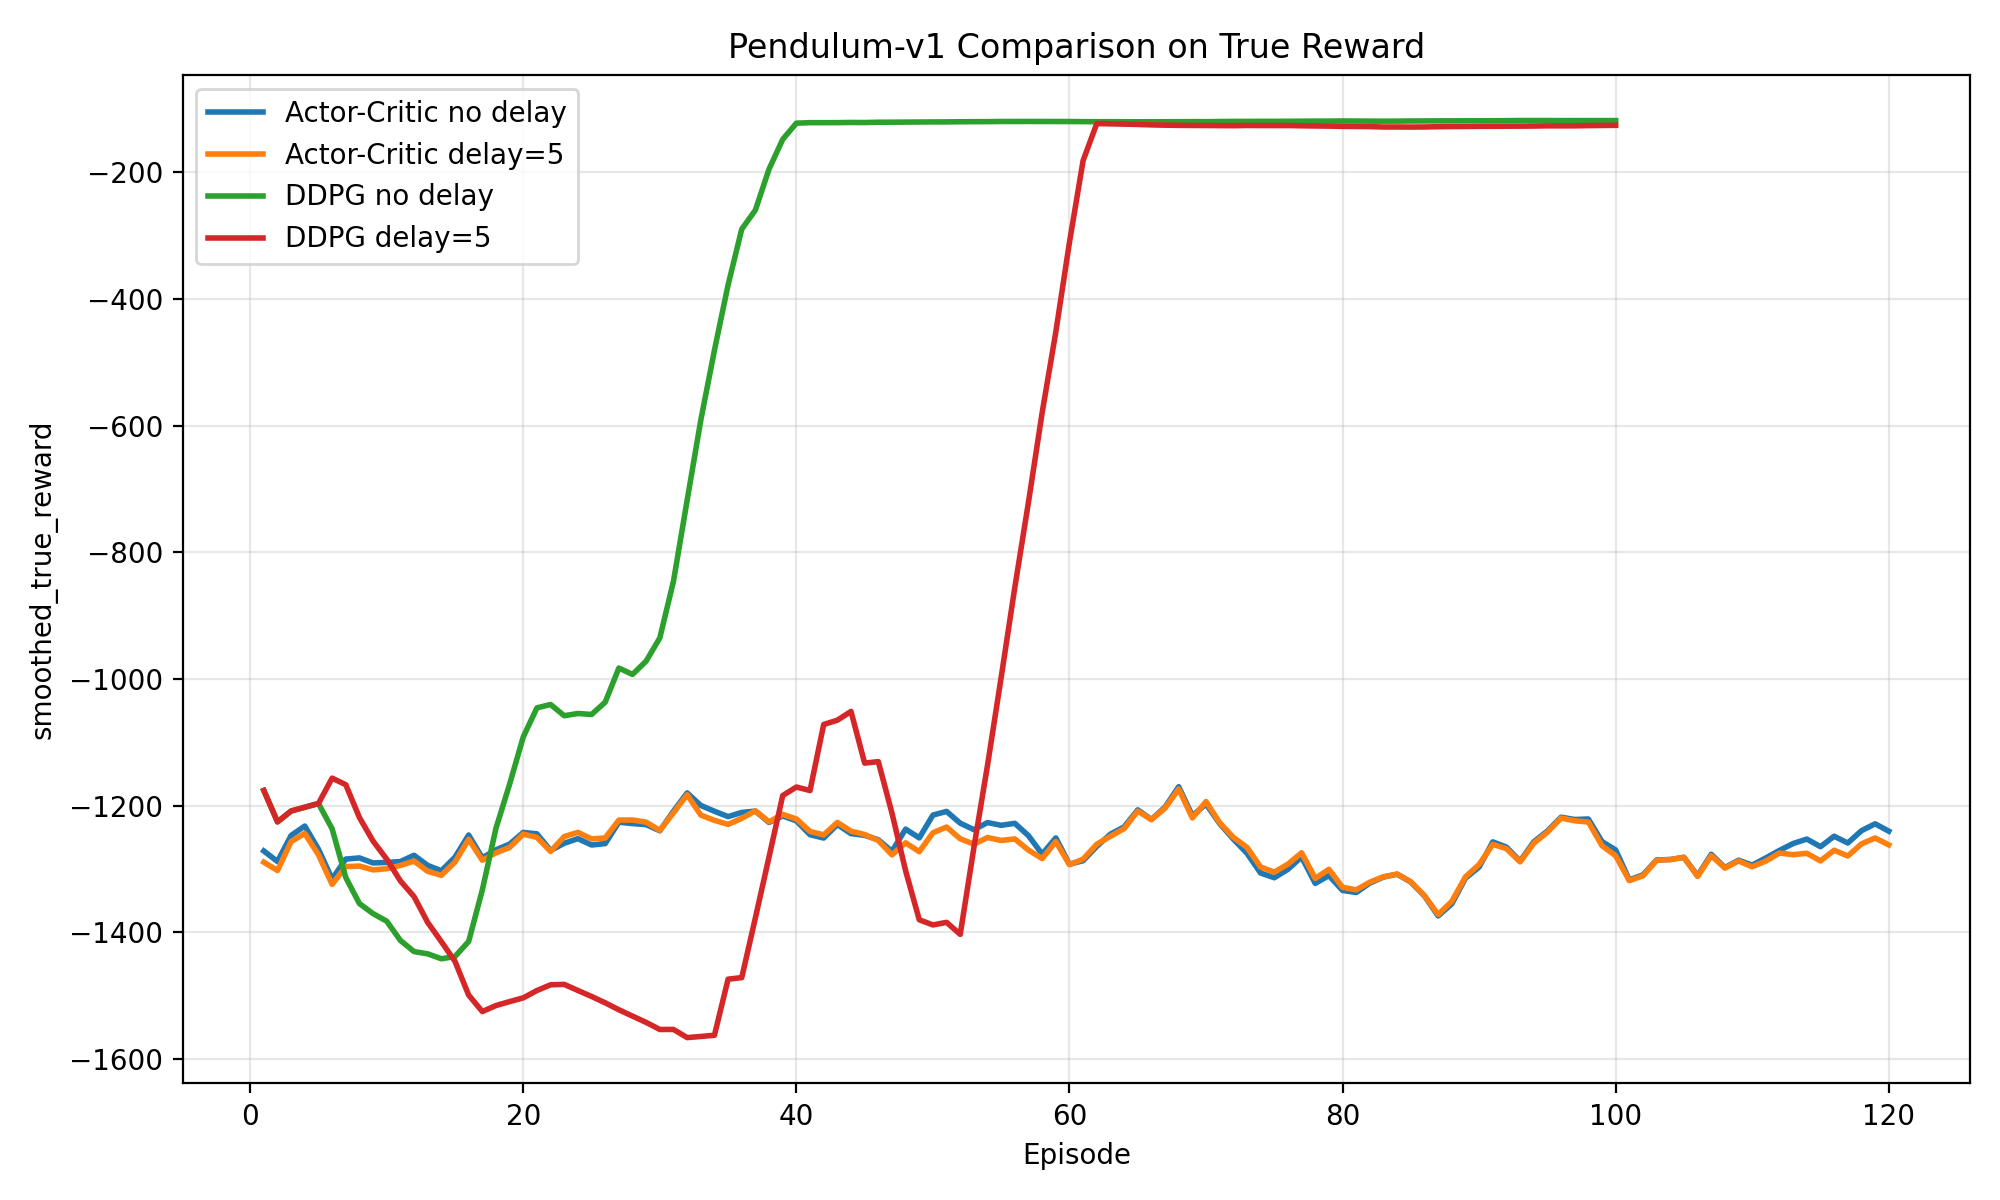
\includegraphics[width=0.92\linewidth]{comparison_true_reward.png}
\caption{四组实验平滑真实回报对比}
\label{fig:comparison}
\end{figure}

\begin{table}[H]
\centering
\caption{四组实验结果汇总}
\label{tab:results}
\begin{tabular}{lcccc}
\toprule
\textbf{实验} & \textbf{最终平滑($\bar{R}$)} & \textbf{最佳平滑} & \textbf{物理含义} & \textbf{收敛？} \\
\midrule
AC delay=0 & $-1240.14$ & $-1170.03$ & 比随机更差（策略误导性收敛） & 否 \\
AC delay=5 & $-1261.85$ & $-1173.58$ & 比随机更差（延迟加剧恶化） & 否 \\
\textbf{DDPG delay=0} & \textbf{$-118.36$} & \textbf{$-118.27$} & 接近最优（$\theta\approx0,\ \tau\approx0$） & \textbf{是} \\
\textbf{DDPG delay=5} & \textbf{$-125.86$} & \textbf{$-123.13$} & 略逊于最优（延迟引入Q值偏差） & \textbf{是} \\
\bottomrule
\end{tabular}
\end{table}

\subsection{DDPG无延迟 vs 5步延迟详细对比}

\begin{figure}[H]
\centering
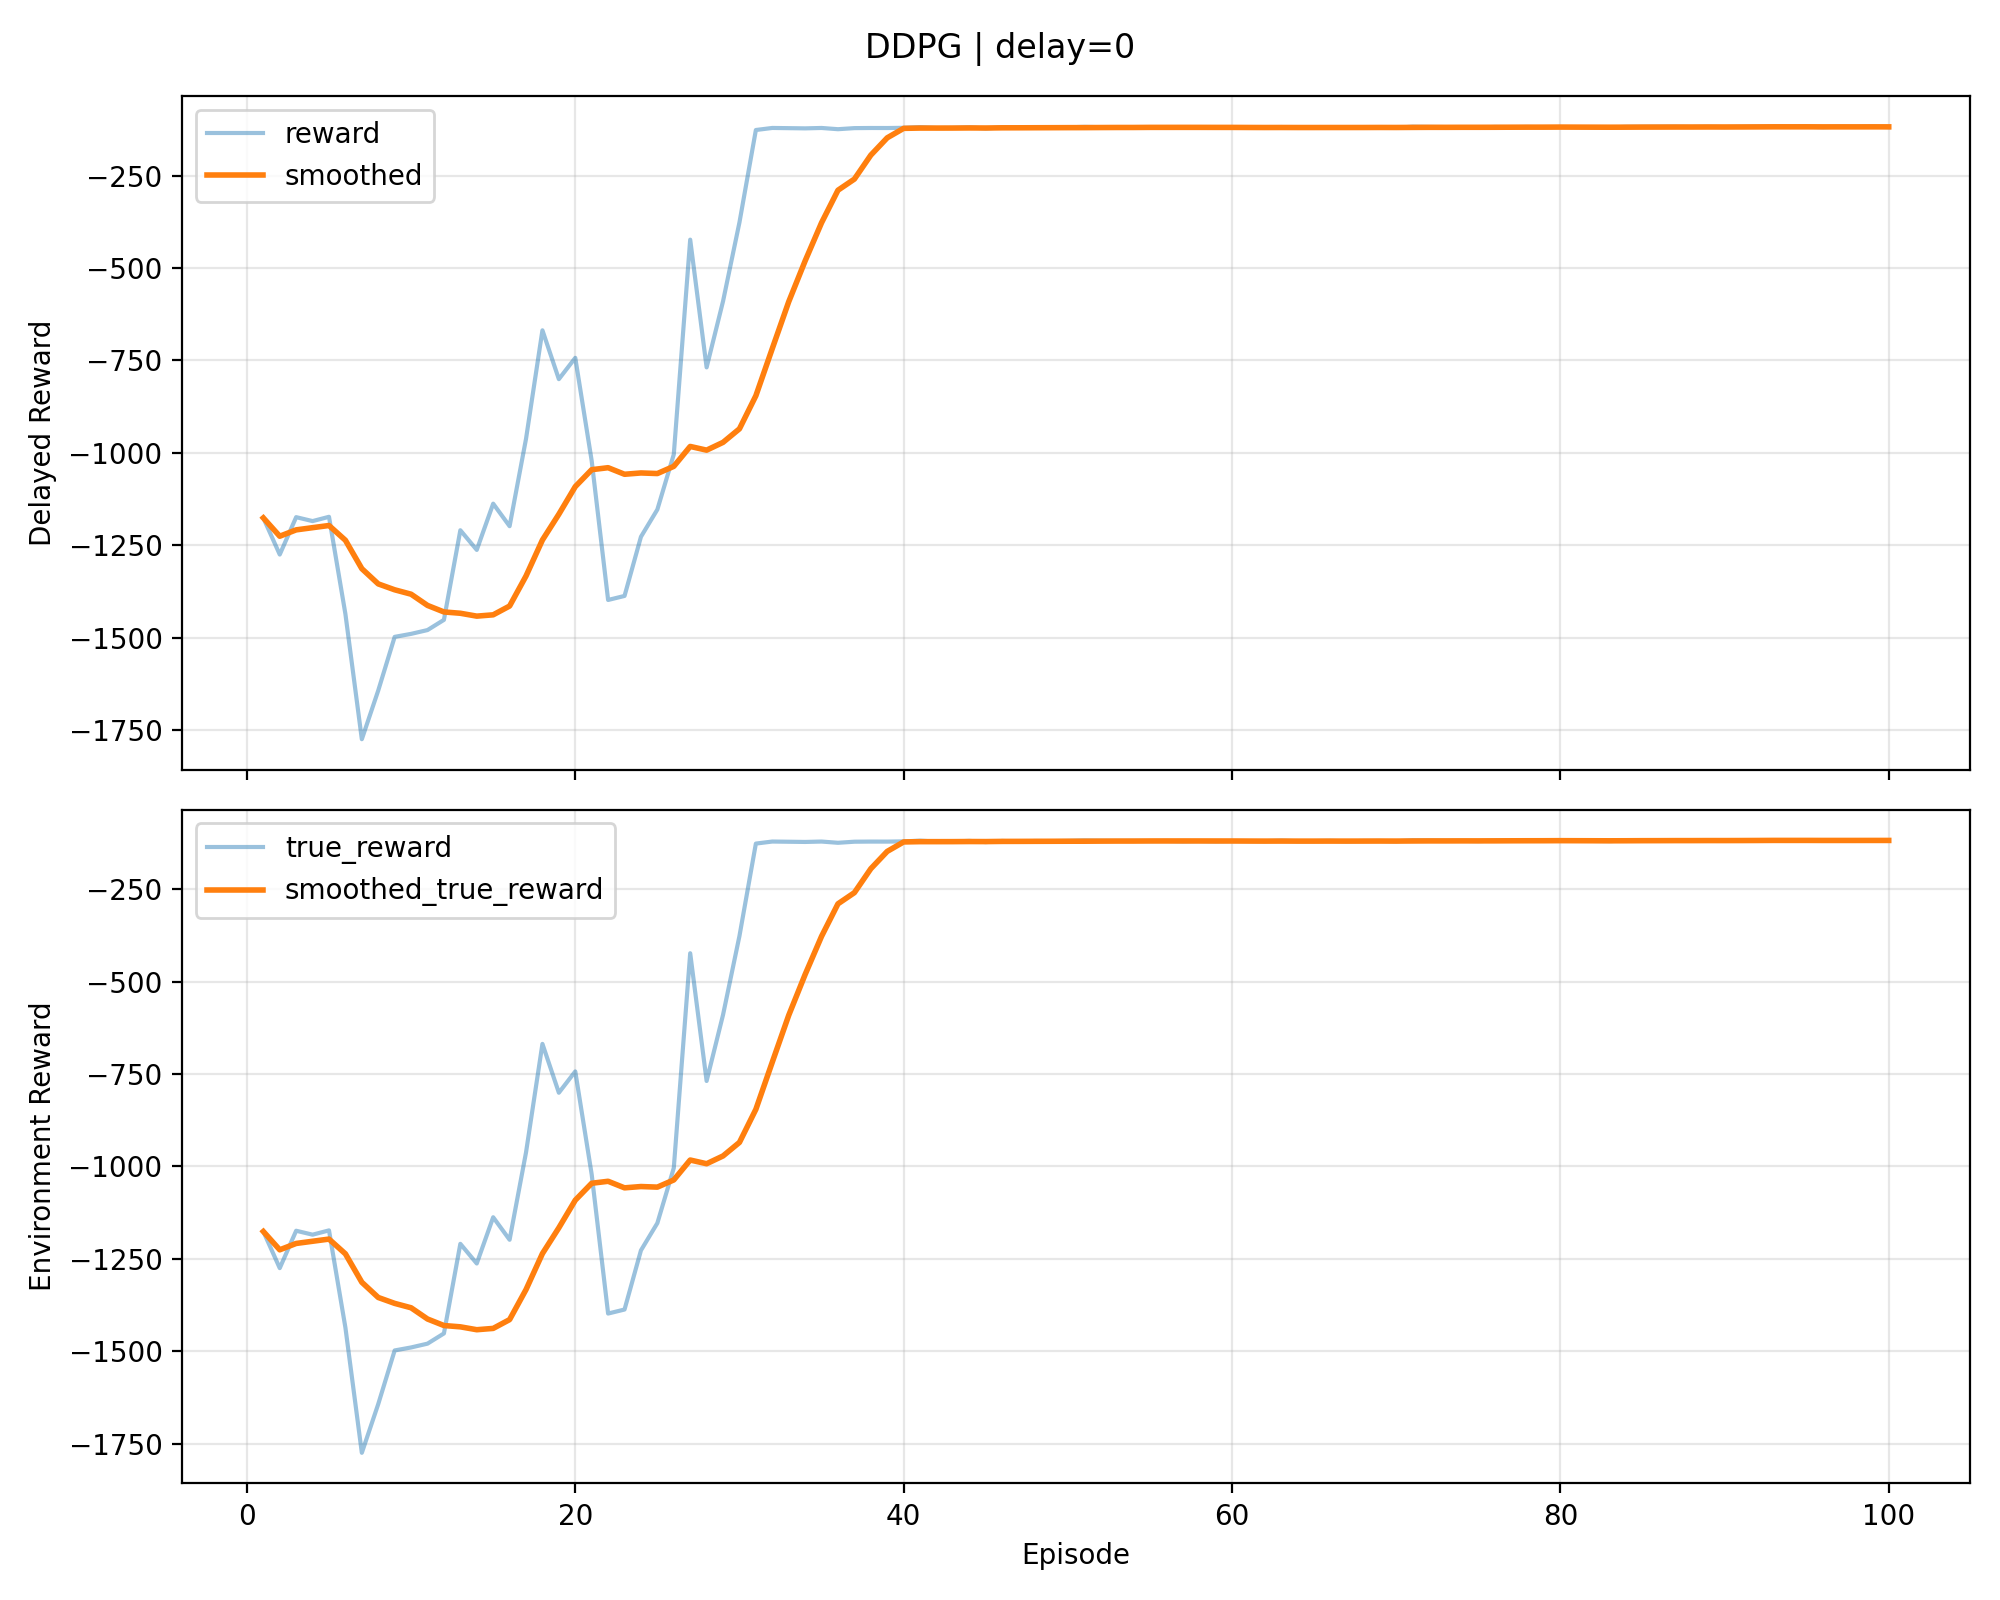
\includegraphics[width=0.92\linewidth]{ddpg_delay0_curve.png}
\caption{DDPG无延迟训练曲线}
\label{fig:ddpg_delay0}
\end{figure}
\begin{figure}[H]
\centering
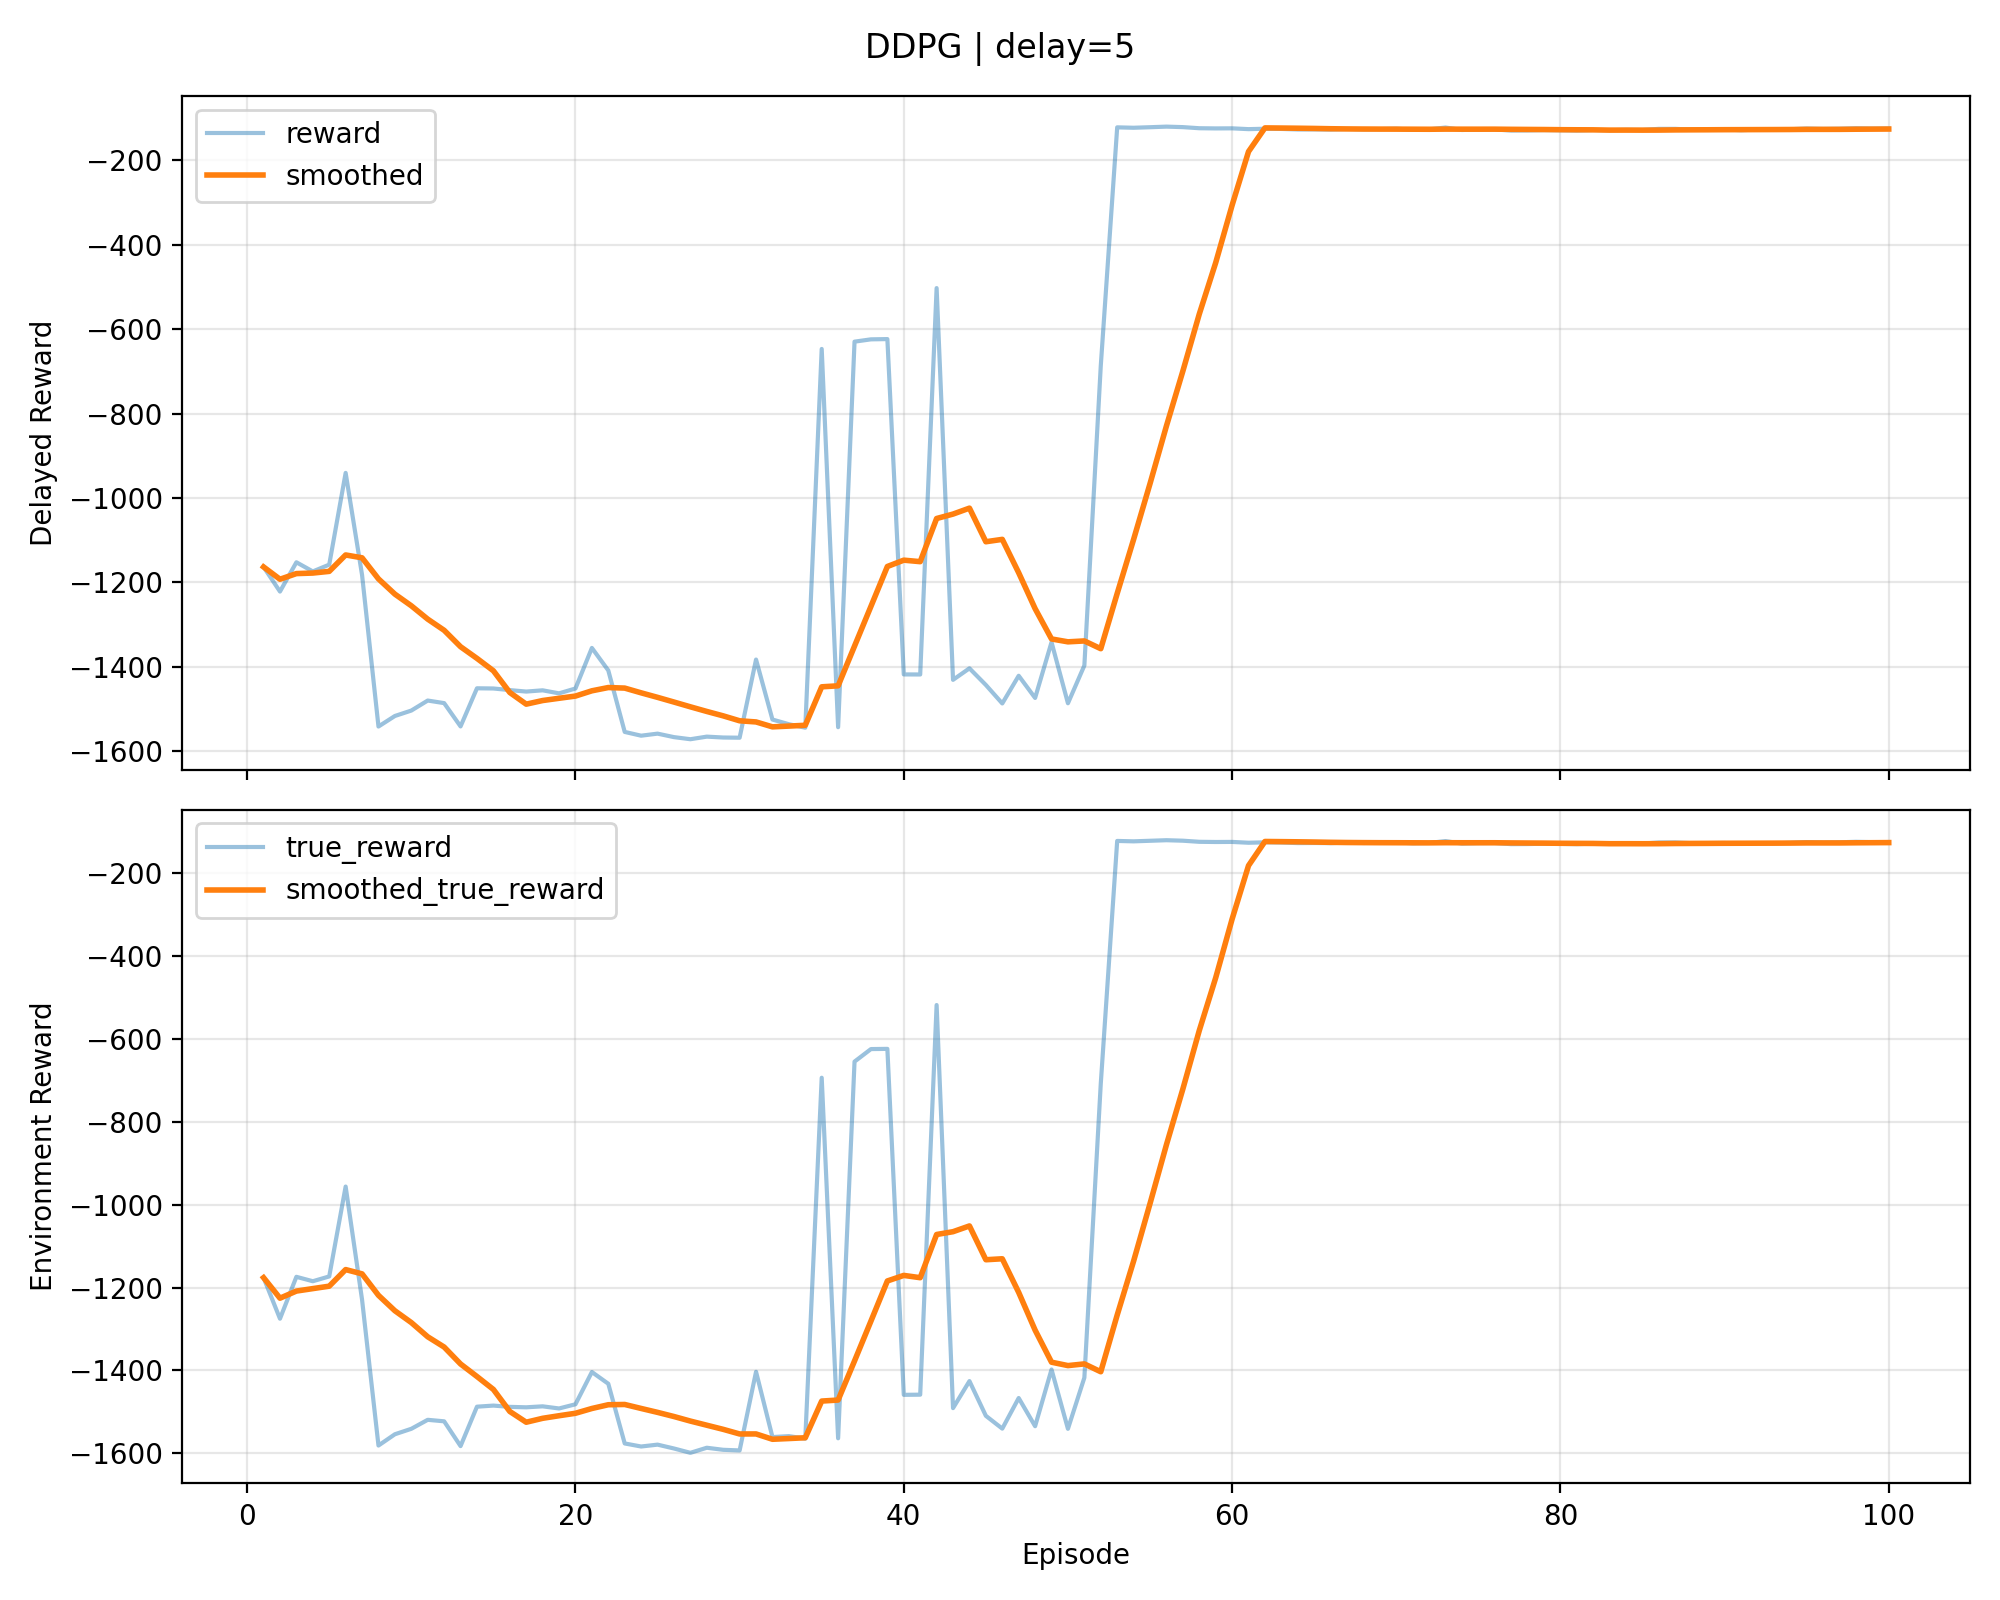
\includegraphics[width=0.92\linewidth]{ddpg_delay5_curve.png}
\caption{DDPG延迟5步训练曲线}
\label{fig:ddpg_delay5}
\end{figure}

\paragraph{收敛速度：}无延迟在第31ep即达$-126.87$；延迟5步要到第53ep才开始显著下降。延迟使探索时间增加约70\%。

\paragraph{最终性能：}无延迟$-118.36$ vs 延迟5步$-125.86$，下降约6.3\%。Critic基于滞后信号拟合Q函数导致值函数偏差。

\paragraph{曲线形态：}无延迟曲线平滑单调下降；延迟5步前52ep在$-1500$和$-120$间反复跳跃，出现"探索-遗忘"现象。

\subsection{Actor-Critic失败分析}

AC在无延迟和延迟5步下均未收敛，累计回报$-1170\sim-1526$（比随机策略$-1084$更差），原因：
\begin{enumerate}[leftmargin=2em]
  \item \textbf{On-policy高方差}：单步TD误差方差大；
  \item \textbf{无经验回放}：每个transition只用一次；
  \item \textbf{连续状态空间}：策略梯度估计方差被进一步放大；
  \item \textbf{错误收敛}：高斯策略的均值可能收敛到推出平衡位置的错误方向，导致比随机更差的回报。
\end{enumerate}

\subsection{DDPG抗延迟鲁棒性}

DDPG在延迟下仍能收敛得益于其off-policy特性：经验回放允许从历史样本中重新学习；目标网络软更新确保学习目标不因延迟剧烈震荡；Critic通过大量经验学到reward的统计规律。

\section{结论}

\begin{enumerate}[leftmargin=2em]
  \item DDPG无延迟收 至$-118.36$，与Keras教程一致且性能更优；
  \item Reward公式为$r=-(\theta^2+0.1\dot\theta^2+0.001\tau^2)$。最优策略$-120$，随机策略$-1080$，据此可判断AC策略比随机更差（$-1240$）；
  \item 5步延迟使DDPG收敛速度减慢70\%，性能下降6.3\%，但最终仍收敛；
  \item AC在两种条件下均不收敛，比随机策略更差的回报说明on-policy学习在高维连续空间中极易陷入错误局部最优；
  \item DDPG的off-policy机制对reward延迟具有天然鲁棒性。
\end{enumerate}

\end{document}